%%
%% cap3.tex
%% 
%% Made by Carlos Calcaneo Roldan
%% Login   <calcaneo@jogrant>
%% 
%% Started on  Mon Jul 22 15:03:25 2019 Carlos Calcaneo Roldan
%% Last update Time-stamp: <2020-jul-29.miércoles 19:05:05 ()>
%%

\chapter{Halos de Materia Oscura}
\setcounter{equation}{0}

%%%%%%%%EL TExto Comienza abajo de aquí! 


\section{Evolución de la cantidad de halos}


En la evolución del Universo, la materia del Universo se comenzó a agrupar lentamente en lo que llamamos halos. En un principio la materia parece una nube difusa sin estructuras internas, después de un tiempo en el que se esta agrumando, pequeñas estructuras de materia se empiezan a formar. Las primeras estructuras son pocas como se aprecia en la figura \ref{fig:EvoNumTotHalos}. Las estructuras tardan tiempo en aparecer y eventualmente hay un aumento acelerado en la cantidad halos que se forman y mas hacia al presente vemos un pico donde empiezan a disminuir el total de halos.

\begin{figure}[ht!]
    \centering
    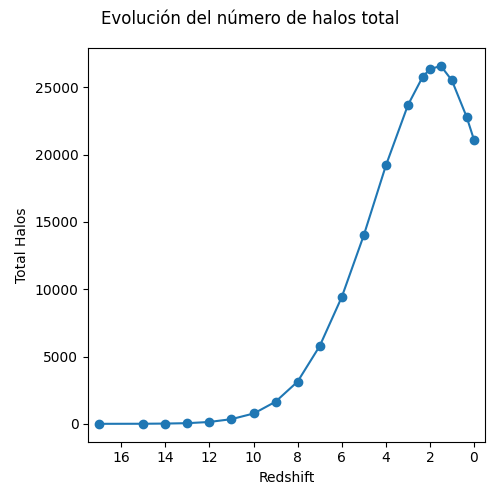
\includegraphics[scale = 0.55]{TotalHalos.png}
    \caption[Evolución del número de halos en un Universo $\Omega_\lambda = 0.691 $, $\Omega_0 = 0.309$]{Se muestra el numero de halos y como cambia la cantidad conforme evoluciona el Universo en una cosmología $\Omega_\lambda = 0.691 $ y $\Omega_0 = 0.309$.}
    \label{fig:EvoNumTotHalos}
\end{figure}

En la figura \ref{fig:MassDistCanonRunSep} podemos observar que aunque disminuyen la cantidad de halos después del redshift 2, podemos ver que comienzan a aparecer estructuras mas masivas. Las estructuras en un principio son pequeñas y escasas y conforme el el Universo evoluciona podemos ver una gran cantidad de halos pequeños a medianos. Mas la presente, se observan que las estructuras son cada vez mas grandes aunque no en gran variedad.

\begin{figure}[ht!]
    \centering
    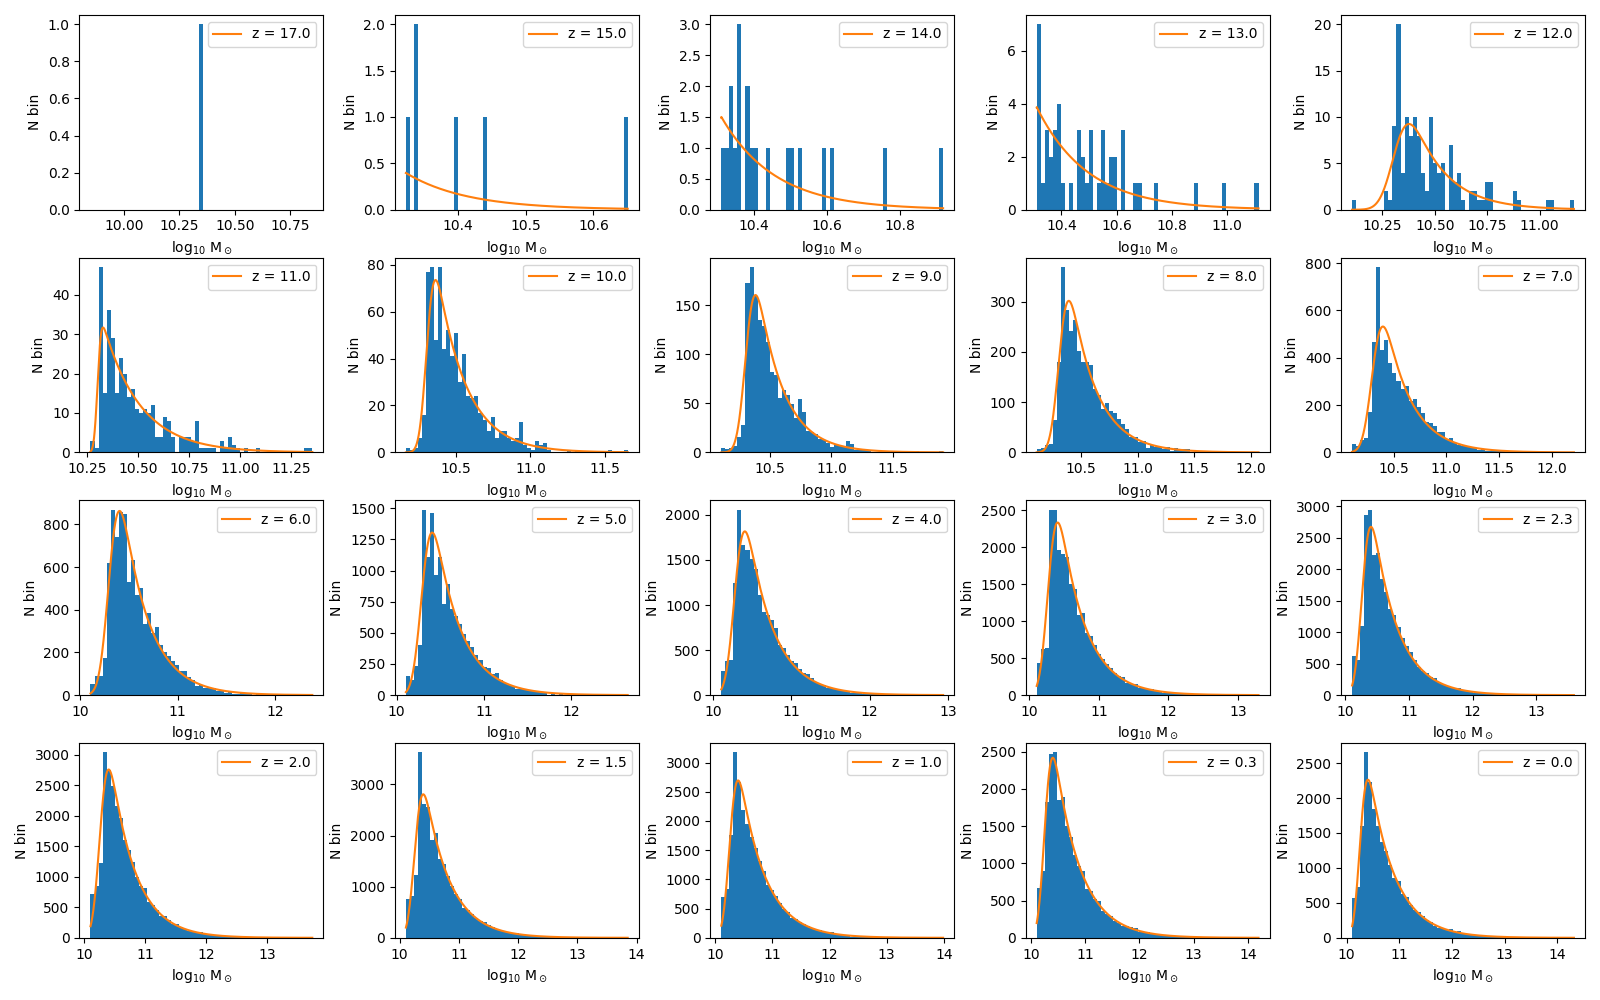
\includegraphics[width = 1\linewidth]{MassDistCanonRunSep.png}
    \caption[Distribución de masa en la evolución de un Universo $\Omega_\lambda = 0.691 $, $\Omega_0 = 0.309$]{Se muestra la distribución de la masa conforme evoluciona el Universo en una cosmología $\Omega_\lambda = 0.691 $ y $\Omega_0 = 0.309$. Se observa como aumentan la cantidad de halos cada vez mas masivos.}
    \label{fig:MassDistCanonRunSep}
\end{figure}



\section{Cúmulo proyectado sobre el plano de S2}


